\documentclass[]{article}
\usepackage{lmodern}
\usepackage{amssymb,amsmath}
\usepackage{ifxetex,ifluatex}
\usepackage{fixltx2e} % provides \textsubscript
\ifnum 0\ifxetex 1\fi\ifluatex 1\fi=0 % if pdftex
  \usepackage[T1]{fontenc}
  \usepackage[utf8]{inputenc}
\else % if luatex or xelatex
  \ifxetex
    \usepackage{mathspec}
  \else
    \usepackage{fontspec}
  \fi
  \defaultfontfeatures{Ligatures=TeX,Scale=MatchLowercase}
\fi
% use upquote if available, for straight quotes in verbatim environments
\IfFileExists{upquote.sty}{\usepackage{upquote}}{}
% use microtype if available
\IfFileExists{microtype.sty}{%
\usepackage{microtype}
\UseMicrotypeSet[protrusion]{basicmath} % disable protrusion for tt fonts
}{}
\usepackage[margin=1in]{geometry}
\usepackage{hyperref}
\hypersetup{unicode=true,
            pdftitle={Chapter 3: Splines},
            pdfborder={0 0 0},
            breaklinks=true}
\urlstyle{same}  % don't use monospace font for urls
\usepackage{graphicx,grffile}
\makeatletter
\def\maxwidth{\ifdim\Gin@nat@width>\linewidth\linewidth\else\Gin@nat@width\fi}
\def\maxheight{\ifdim\Gin@nat@height>\textheight\textheight\else\Gin@nat@height\fi}
\makeatother
% Scale images if necessary, so that they will not overflow the page
% margins by default, and it is still possible to overwrite the defaults
% using explicit options in \includegraphics[width, height, ...]{}
\setkeys{Gin}{width=\maxwidth,height=\maxheight,keepaspectratio}
\IfFileExists{parskip.sty}{%
\usepackage{parskip}
}{% else
\setlength{\parindent}{0pt}
\setlength{\parskip}{6pt plus 2pt minus 1pt}
}
\setlength{\emergencystretch}{3em}  % prevent overfull lines
\providecommand{\tightlist}{%
  \setlength{\itemsep}{0pt}\setlength{\parskip}{0pt}}
\setcounter{secnumdepth}{5}
% Redefines (sub)paragraphs to behave more like sections
\ifx\paragraph\undefined\else
\let\oldparagraph\paragraph
\renewcommand{\paragraph}[1]{\oldparagraph{#1}\mbox{}}
\fi
\ifx\subparagraph\undefined\else
\let\oldsubparagraph\subparagraph
\renewcommand{\subparagraph}[1]{\oldsubparagraph{#1}\mbox{}}
\fi

%%% Use protect on footnotes to avoid problems with footnotes in titles
\let\rmarkdownfootnote\footnote%
\def\footnote{\protect\rmarkdownfootnote}

%%% Change title format to be more compact
\usepackage{titling}

% Create subtitle command for use in maketitle
\newcommand{\subtitle}[1]{
  \posttitle{
    \begin{center}\large#1\end{center}
    }
}

\setlength{\droptitle}{-2em}

  \title{Chapter 3: Splines}
    \pretitle{\vspace{\droptitle}\centering\huge}
  \posttitle{\par}
    \author{}
    \preauthor{}\postauthor{}
    \date{}
    \predate{}\postdate{}
  

\begin{document}
\maketitle

{
\setcounter{tocdepth}{2}
\tableofcontents
}
\section{Problem 1}\label{problem-1}

\subsection{a. Determine whether the function is a linear
spline}\label{a.-determine-whether-the-function-is-a-linear-spline}

Let's check the properties. First of all it does have a degree of 1 or
less on each piece of the polynomial, so that property passes. Next
let's check for continuity on the inner knots.

At x = 0.5, \(S_0(0.5) = 0.5\) and \(S_1(0.5) = 0.5 = 2 * 0 = 0.5\).
Continuous here.

At x = 2, \(S_1(2) = 0.5 + 2 * 1.5 = 3.5\) and \(S_2(2)=2 + 1.5 = 3.5\).
Continuous here.

This function S(x) must then be a linear spline.

\subsection{b. Do there exist a,b,c,d so the function is a natural cubic
spline?}\label{b.-do-there-exist-abcd-so-the-function-is-a-natural-cubic-spline}

Recall that a natural cubic spline uses the condition that the second
derivative at the end knots both equal to zero.

Let's set up our system:

\[S_0''(-1) = 6ax + 2 = 0\] \[-6a = -2\] \[a = \frac23\]

\[S_1''(1) = 6bx + 2 = 0\] \[6b = -2\] \[b = -\frac23\]

So yes, there do exist an a,b,c, and d so the function is a natural
cubic spline. If a = 2/3 and b = -2/3, then the two end points are
points of inflection.

\subsection{c. Determine whether f is a cubic spline with knots -1, 0,
1, and
2}\label{c.-determine-whether-f-is-a-cubic-spline-with-knots--1-0-1-and-2}

First of all we can confirm that each piece of the function is degree 3
or less. Second let's test for continuity between knots.

At 0:

\[S_0(0) = S_1(0)\] \[1 + 2(0+1) + (0+1)^3=3+5*0+3*0\] \[1 + 2 + 1 = 3\]
\[3 = 3\]

That works, next at 1:

\[S_1(1) = S_2(1)\] \[3 + 5 + 3 = 11 + 0 + 3 * 0 + 0\] \[11 = 11\]

That works, check first derivative at 0:

\[S_0'(0) = S_1'(0)\] \[2+3(0+1)^2=5 + 6 * 0\] \[2 + 3 = 5\] \[5 = 5\]

That works, next at 1:

\[S_1'(1) = S_2'(1)\] \[5 + 6 * 1 = 6(1-1)+3(1-1)^2+1\] \[5 \ne 1\]

Therefore the function f is NOT a cubic spline, since it is not (k-1)
times differntiable at it's inner knots.

\subsection{d. Determine the values of a,b,c such that the function is a
linear
spline.}\label{d.-determine-the-values-of-abc-such-that-the-function-is-a-linear-spline.}

Let's create our system of equations (for three unknowns).

\[S_0(-1) = s_1(-1)\] \[S_1(0) = S_2(0)\] \[S_2(1) = s_3(1)\]

Now let's solve one at a time from the end.

\[c(1) + 3(1-1) = 4\] \[c = 4\]

Now that we know c is four let's move to the second equation.

\[a(0 + 1) + b * 0 = 4 * 0 + 3(0-1)\] \[a = -3\]

Then move on to our first equation we wrote.

\[-3(-1 + 1) + b * -1 = -1 + 1\] \[-b = 0\] \[b = 0\]

So we can conclude taht a = -3, b = 0, and c = 4 gives us a linear
spline.

\subsection{e. Determine the values of a,b,c such that the function is a
linear
spline.}\label{e.-determine-the-values-of-abc-such-that-the-function-is-a-linear-spline.}

Let's create our system of equations (for three unknowns).

\[S_0(-1) = s_1(-1)\] \[S_1(0) = S_2(0)\] \[S_2(1) = s_3(1)\]

Now let's solve one at a time from the the end.

\[c(1) + 2(1-1) = 5\] \[c = 5\]

Now we know c is five let's move to the second equation.

\[a(0+1) + b * 0 = 5*0 + 2(0-1)\] \[a=-2\]

Then move on to our first equation we wrote.

\[-1 + 3 = -2(-1 + 1) + b * -1\] \[2 = -b\] \[b=-2\]

So we can conclude that a = b = -2, and c = 5 gives us a linear spline.

\section{Problem 2}\label{problem-2}

Given a set of data

\[
\begin{tabular}{c|c|c|c|c|c}
t$_i$ & 1.2 & 1.5 & 1.6 & 2.0 & 2.2\\
y$_i$ & 0.4275 & 1.139 & 0.8736 & -0.9751 & -0.1536
\end{tabular}
\]

\subsection{a.}\label{a.}

Let L(x) be the linear spline that interpolates the data. Describe what
L(x) consists of, and what conditions it has to satisfy. Find L(x), and
compute the value for L(1.8).

There are two main conditions a linear spline would have to fulfill. It
would have to be of degree 1 polynomial on each piece, and L(x) would
have to be continous at each knot denoted in the table.

For a linear spline we can just use the equation of a linear point as
written:

\[S_i(x) = y_i + \frac{y_{i+1}-y_i}{t_{i+1}-t_i}(x-t_i)\]

For i = 0:

\[S_0(x) = 0.4275 + \frac{1.139 - 0.4275}{1.5-1.2}(x-1.2)\]
\[S_0(x) = 0.4275 + 2.3717(x-1.2)\]

For i = 1

\[S_1(x) = 1.139 + \frac{0.8736 - 1.139}{1.6-1.5}(x-1.5)\]
\[S_1(x) = 1.139 - 2.654(x-1.5)\]

For i = 2

\[S_2(x) = 0.8736 + \frac{-0.9751 - 0.8736}{2.0-1.6}(x-1.6)\]
\[S_2(x) = 0.8736 - 4.6218(x-1.6)\]

For i = 3

\[S_3(x) = -0.9751 + \frac{-0.1536 + 0.9751}{2.2-2.0}(x-2.0)\]
\[S_3(x) = -0.9751 + 4.1075(x-2.0)\]

\[
S(x) = \left\{
        \begin{array}{ll}
            0.4275 + 2.3717(x-1.2) & \quad 1.2 \leq x \leq 1.5 \\
            1.139 - 2.654(x-1.5) & \quad 1.5 \leq x \leq 1.6 \\
            0.8736 - 4.6218(x-1.6) & \quad 1.6 \leq x \leq 2.0\\
            -0.9751 + 4.1075(x-2.0) & \quad 2.0 \leq x \leq 2.2
        \end{array}
    \right.
\]

\[S(1.8) = S_2(1.8) = 0.8736 - 4.6218(1.8 - 1.6) =  -0.05076\]

\subsection{b.}\label{b.}

Let C(x) be the natural cubic spline that interploates the data.
Describe what C(x) consists of, and what conditions it has to satisfy.
Find C(x), and compute the value for C(1.8). The computation here can be
time consuming, and you may use Matlab to solve the linear system.

C(x) is a piecewise function that consists of 4 3rd degree polynomials.
The fuction C(x) must be continous up to twice differentiable. In our
case we our looking for a natural cubic spline, so the end points must
have a second derivative of zero.

\[
S(x) = \left\{
        \begin{array}{ll}
            -18.8675x^3+4.0697x+0.4275 & \quad 1.2 \leq x \leq 1.5 \\
            6.8546x^3-16.9807x^2-1.0245x+1.1390 & \quad 1.5 \leq x \leq 1.6 \\
            34.7685x^3-14.9243x^2-4.2150x+0.8736 & \quad 1.6 \leq x \leq 2.0\\
            -44.6632x^3+26.7979x^2+0.5344x-0.9751 & \quad 2.0 \leq x \leq 2.2
        \end{array}
    \right.
\]

C(1.8) = -0.2882

\section{Problem 3}\label{problem-3}

Write a Matlab function that computes the linear spline interpolation
for a given data set. You might need to take a look at the file
cspline\_eval.m in section 3.4 for some hints. Name your Matlab function
lspline. This can be defined in the file lspline.m.

Use your Matlab function lspline on the given data set in Problem 2,
plot the linear spline for the interval {[}1.2, 2.2{]}.

Matlab function:

\begin{verbatim}
function S = cspline_eval(t,y,z,x_vec)
% function S = cspline_eval(t,y,z,x_vec)
% compute the value of the natural cubic spline at the points x_vec when
% t,y,z are given
%
% Example:   t = [0.9,1.3,1.9,2.1];
%            y = [1.3,1.5,1.85,2.1]
%            z = cspline(t,y)
%            x = [0.9:0.1:2.1]
%            v = cspline_eval(t,y,z,x)

m = length(x_vec);
S = zeros(size(x_vec));  
n = length(t);
for j=1:m
  x = x_vec(j);
  for i=n-1:-1:1
    if (x-t(i)) >= 0
      break
    end
  end
  h = t(i+1)-t(i);
  S(j) = z(i+1)/(6*h)*(x-t(i))^3-z(i)/(6*h)*(x-t(i+1))^3 ...
       +(y(i+1)/h-z(i+1)*h/6)*(x-t(i)) - (y(i)/h-z(i)*h/6)*(x-t(i+1));
end
\end{verbatim}

Input/Output:

lspline(t,y,t)

ans =

\begin{quote}
\begin{quote}
0.4275 1.1390 0.8736 -0.9751 -0.1536
\end{quote}
\end{quote}

x = {[}1.4 1.5 1.6 1.7 1.8{]};

lspline(t,y,x)

ans =

\begin{quote}
\begin{quote}
0.9018 1.1390 0.8736 0.4114 -0.0508
\end{quote}
\end{quote}

Which this 1.8 value is the same we got when manually evaluating the
spline.

Script to make plot:

\begin{verbatim}
x = 1.2:0.1:2.2;
t = [1.2 1.5 1.6 2.0 2.2];
y = [0.4275 1.139 0.8736 -0.9751 -0.1536];

yVals = lspline(t,y,x);

figure
plot(x,yVals)
grid on
xlabel('Chosen Points')
ylabel('Linear Spline Points')
\end{verbatim}

And the plot! If you compared adding extra points in the plot, that it
does not change what is plotted, because you maintain the piecewise
linear plot.

\begin{figure}
\centering
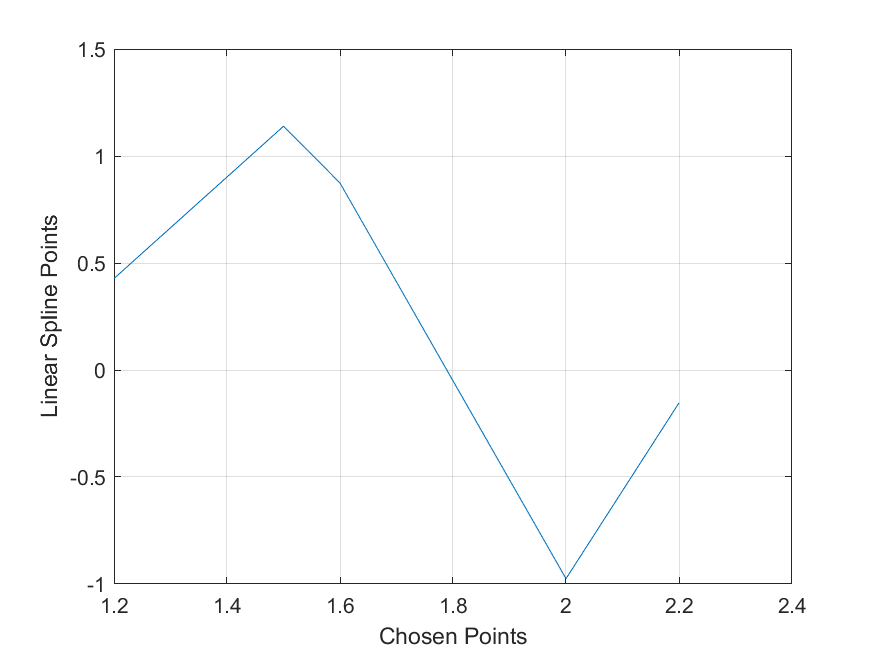
\includegraphics{./Media/problem3Plot.png}
\caption{}
\end{figure}

\section{Problem 4}\label{problem-4}

I made a script that allows you to click the points on a screenshot of
the image and it uses those points to run the spline interpolation that
is then plotted. I clicked a series of twenty points, and more near the
top in hopes that a higher resolution would make the top of the mountain
sharper, since we konw that the cubic spline generates the smoothest
interpolation. The peak does appear in the plot. I am including both the
plot of the points and the Matlab printout of the points I clicked.

\begin{verbatim}
% display image
everest = imread('../Media/mountEverest.png');
image(everest)
grid on

% click knot points
[t, y] = ginput(20);
y = y.*-1;

z = cspline(t, y);

min = t(1);
max = t(20);
x = min:0.001:max;

yPlot = cspline_eval(t, y, z, x);

figure
plot(x, yPlot)
xlabel('Range of clicked points')
ylabel('Interpolated Points')
title('Interpolated ridge')
\end{verbatim}

The points (x, y):

\begin{itemize}
\tightlist
\item
  10.3318 -207.3163
\item
  32.3088 -188.9490
\item
  61.2258 -166.9082
\item
  95.9263 -141.1939
\item
  128.3134 -115.4796
\item
  173.4240 -81.6837
\item
  197.7143 -62.5816
\item
  212.7512 -52.2959
\item
  239.3548 -42.7449
\item
  252.0783 -44.9490
\item
  272.8986 -47.1531
\item
  287.9355 -61.1122
\item
  316.8525 -80.9490
\item
  337.6728 -110.3367
\item
  361.9631 -154.4184
\item
  373.5300 -186.7449
\item
  378.1567 -182.3367
\item
  389.7235 -173.5204
\item
  411.7005 -155.8878
\item
  462.5945 -218.3367
\end{itemize}

\begin{figure}
\centering
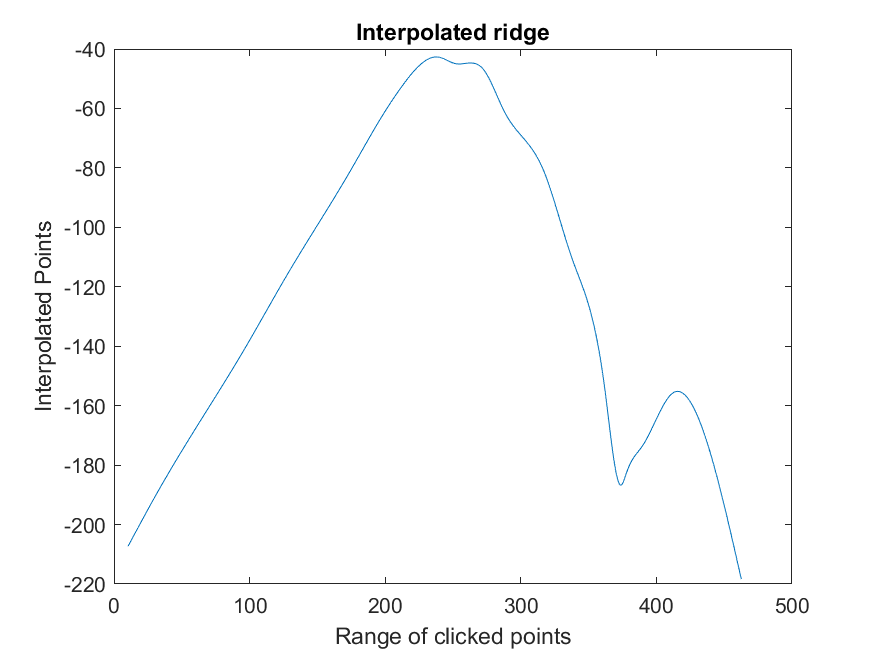
\includegraphics{./Media/mountEverestPlot.png}
\caption{}
\end{figure}


\end{document}
